%\documentclass[10pt,a4paper]{IEEEtran}
%\usepackage[latin1]{inputenc}
%\usepackage{amsmath}
%\usepackage{amsfonts}
%\usepackage{amssymb}
%\usepackage{graphicx}
%\begin{document}

\section{Quantile Autoregression}

Our main objective in this paper is estimating the p-step ahead $\alpha$-quantile function $\mathcal{Q}_{y_t|y_{t-p}}^\alpha(t)$ for a given set of time series data $y_t$, as the one on figure \ref{fig:exemployt}. So, given a sequence $\{y_t\}$, we can pair an observation $y_t$ with its $p$-lagged correspondent $y_{t-p}$. Figure \ref{fig:exemploar} shows this relationship. We will assume that all information regarding the estimated quantile value are past observations, being in accordance with other pure autoregressive models.  

\begin{figure}[h]
\centering
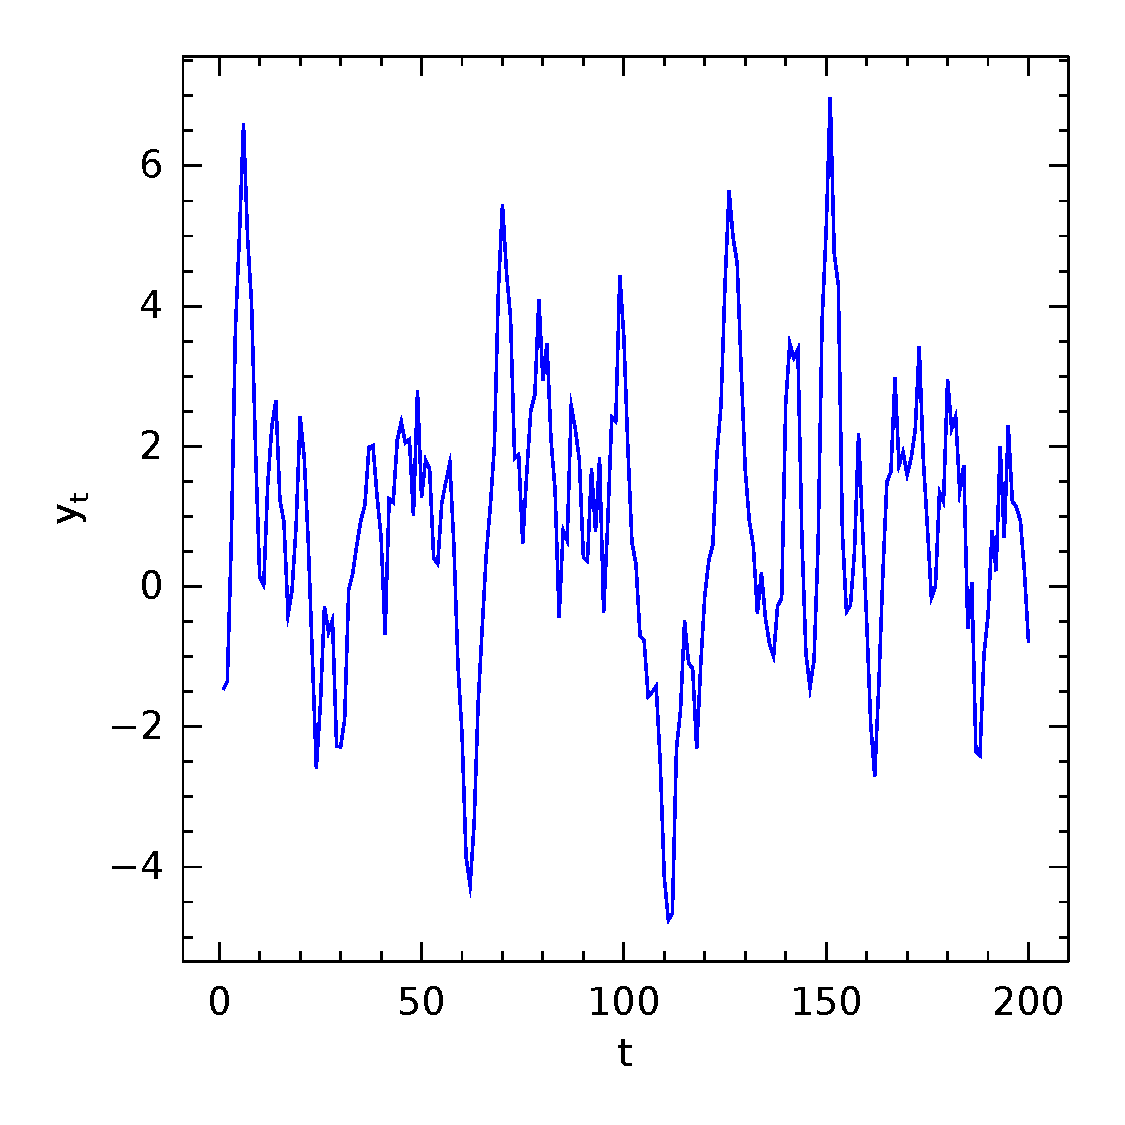
\includegraphics[width=0.7\linewidth]{Figuras/exemplo-yt}
\caption{Time series $y_t$}
\label{fig:exemployt}
\end{figure}

\begin{figure}[h]
\centering
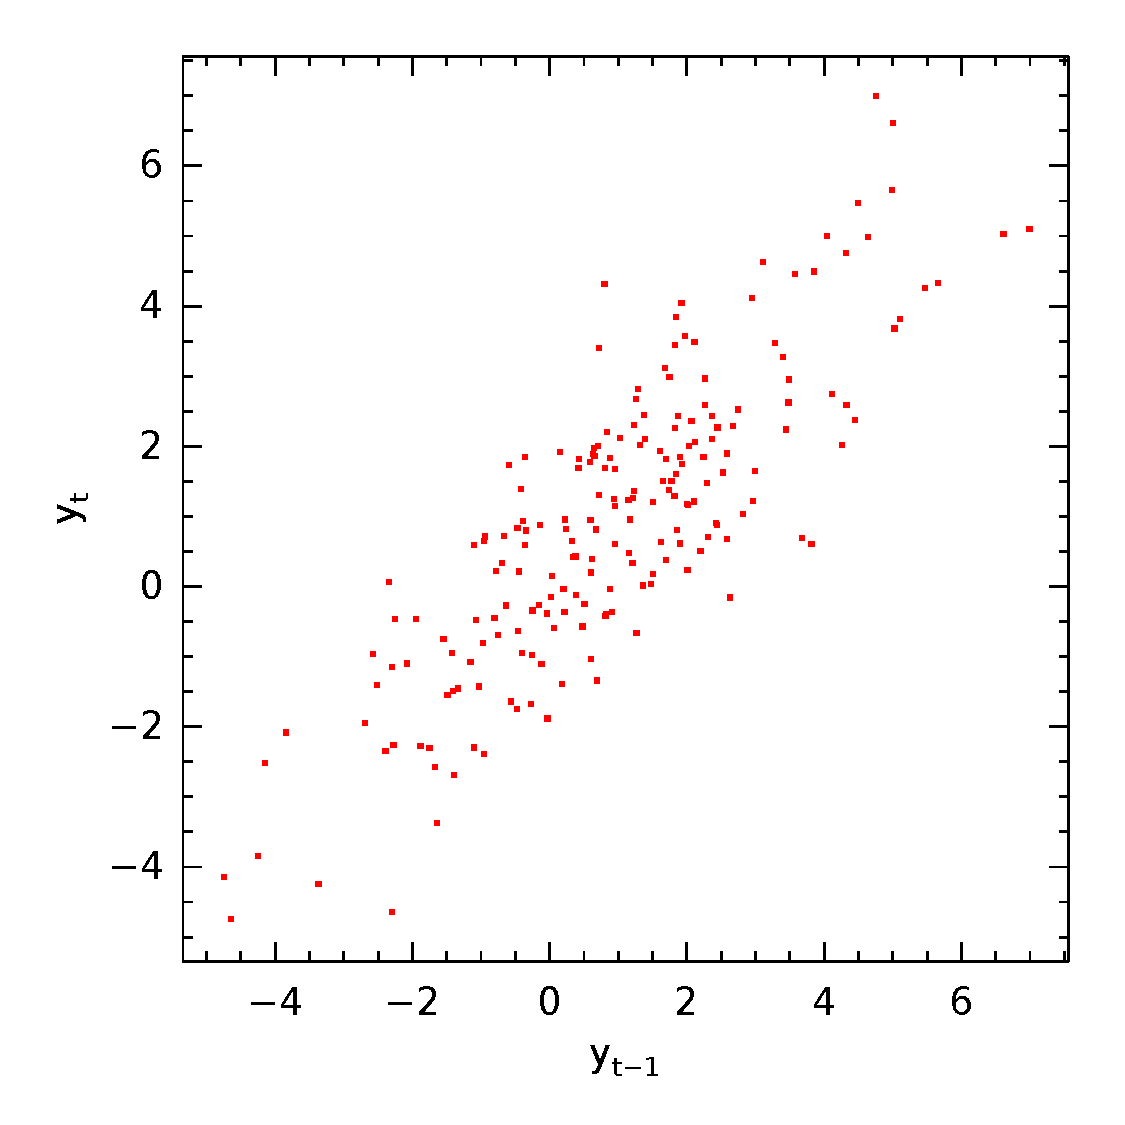
\includegraphics[width=0.7\linewidth]{Figuras/exemplo-ar}
\caption[Tst]{Relationship between $y_t$ and its first lag $y_{t-1}$}
\label{fig:exemploar}
\end{figure}

We will investigate two ways of estimating the quantiles for the aforementioned relationship: we will use a linear and a nonparametric model.

\section{Linear-QAR}



\section{NP-QAR}

Fitting a linear estimator for the Quantile Auto Regression isn't appropriate  when nonlinearity is present in the data. This nonlinearity may produce a linear estimator that underestimates the quantile for a chunk of data while overestimating for the other chunk (we illustrate this in figure \ref{fig:nonlinear}). To prevent this issue from occurring we propose a modification which we let the prediction $\mathcal{Q}_{y_t|y_{t-1}}^\alpha(t)$ adjust freely to the data and its nonlinearities. To prevent overfitting and smoothen our predictor, we include a penalty on its roughness by including the $\ell_1$ norm of its second derivative. For more information on the $\ell_1$ norm acting as a filter, one can refer to \cite{kim2009ell_1}.

\begin{figure}
\centering
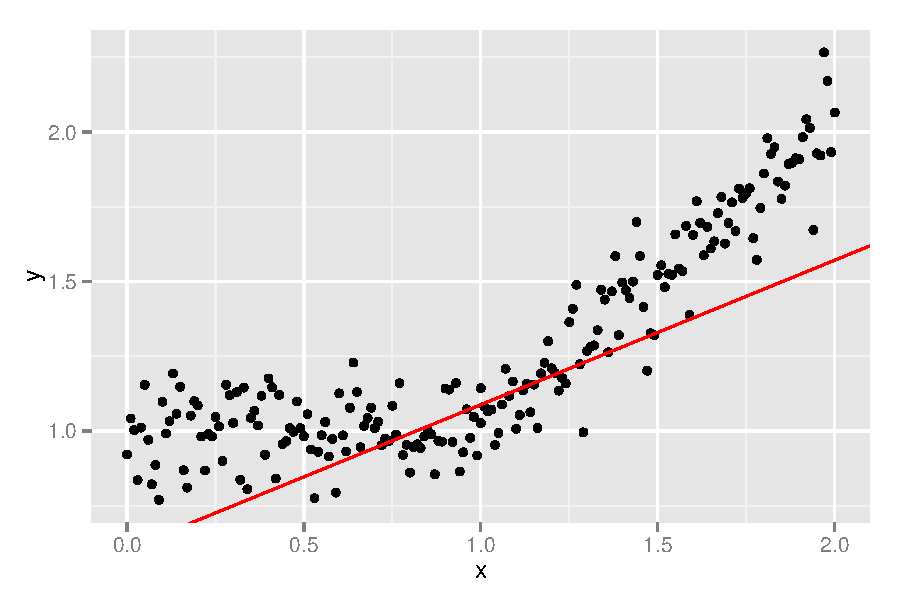
\includegraphics[width=0.7\linewidth]{../Paper_IEEE/nonlinear}
\caption{Example of data where nonlinearity is present and a linear quantile estimator is employed}
\label{fig:nonlinear}
\end{figure}


% nota��o estat�stica de ordem. com x^(0)

Let $\{\tilde{y}_t \}_{t=1}^n$ be the sequence of observations in time $t$. Now, let $\tilde{x}_t$ be the $p-$lagged time series of $\tilde{y}_t$, such that $\tilde{x}_t = L^p(\tilde{y}_t)$, where $L$ is the lag operator. Matching each observation $\tilde{y}_t$ with its $p-$lagged correspondent $\tilde{x}_t$ will produce $n-p$ pairs $\{(\tilde{y}_t,\tilde{x}_t)\}_{t=p+1}^n$ (note that the first $p$ observations of $y_t$ must be discarded). Consider $J$ to be the set of indexes such that
$$\tilde{x}_{J_1} \leq \tilde{x}_{J_2} \leq \dots \leq \tilde{x}_{J_{n-P}}.$$ 
Now, we define $\{x_i\}_{i=1}^{n-p} = \{\tilde{x}_{J_t} \}_{t=p+1}^{n}$ and $\{y_i\}_{i=1}^{n-p} = \{\tilde{y}_{J_t} \}_{t=p+1}^{n}$ and $I = \{2,\dots, n-p-1\}$. As we need the second difference of $q_i$, $I$ has to be shortened by two elements.

Our optimization model to estimate the nonparametric quantile is as follows:
\begin{equation}
\begin{split}
\mathcal{Q}_{y_t|y_{t-1}}^\alpha(i) =\underset{q_{i}}{\arg\min}\sum_{i\in I}\left(|y_{i}-q_{i}|^{+}\alpha + |y_{i}-q_{i}|^{-}(1-\alpha)\right) \\ +\lambda  \sum_{i\in I}|D^{2}q_{i}|,
\end{split}
\end{equation}
where $D^2 q_t$ is the second derivative of the $q_t$ function, calculated as follows:
\begin{equation*}
D^{2}q_{i}=\left(\frac{q_{i+1}-q_{i}}{x_{i+1}-x_{i}}\right)-\left(\frac{q_{i}-q_{i-1}}{x_{i}-x_{i-1}}\right).
\end{equation*}
The first part on the objective function is the usual quantile regression condition for $\{q_i\}$. The second part is the $\ell_1$-filter. The purpose of a filter is to control the amount of variation for our estimator $q_i$. When no penalty is employed we would always get $q_i = y_i$. On the other hand, when $\lambda \rightarrow \infty$, our estimator approaches the linear quantile regression.

The output of our optimization problem is a sequence of ordered points $\{(x_i, q_i)\}_{i \in I}$. The next step is to interpolate these points in order to provide an estimation for any other value of x. To address this issue, we propose a B-splines interpolation, that will be discussed in another subsection.

When estimating quantiles for a few different values of $\alpha$, however, sometimes we find them overlapping each other, which we call crossing quantiles. To prevent this, we include a non-crossing constraint:
\begin{equation}
q_i^{\alpha} \leq q_i^{\alpha'}, \quad \forall i \in I, \alpha < \alpha'.
\end{equation} 

%A seguir, apresentaremos alguns resultados para quando o 

%The difference between using or not this constraint can be seen in the two plots below:
%
%
%
%\bibliography{QR}
%\bibliographystyle{ieeetr}
%
%\end{document}